\chapter{Introduction}
\label{chap:intro}

\section{Motivation}
\label{chap:motivation}

These days witness the development of information extraction methods, which are fruitfully exploited for automatic construction of KGs, that is, a large collection of relational facts with the format $\langle subject \rangle \langle predicate \rangle \langle object \rangle$. These are triples reflecting facts about the real world which can be converted to facts over unary and binary relations in predicate calculus. Every such triple can be represented as a binary fact \textit{predicate(subject, object)} if \textit{predicate} is not \textit{type} and a unary fact \textit{object(subject)} otherwise. For example, $\langle Brad \rangle \langle livesIn \rangle \langle Berlin \rangle$ can be rewritten as $livesIn(Brad, Berlin)$ while $\langle Mat \rangle \langle type \rangle \langle artist \rangle$ can be converted to $artist(Mat)$. Examples of KGs include the YAGO~\cite{ref28}, FreeBase~\footnote{\url{https://developers.google.com/freebase/}}, etc (see Chapter~\ref{chap:relwork} for details).

KGs are normally incomplete due to automatic construction. Hence, they should be processed under the Open World Assumption (OWA). The \textit{knowledge completion problem} (also known as \textit{link prediction}) plays an important role in improving the quality of KGs. To achieve this, rule learning approaches~\cite{ref39, ref10} are used to create rules which can infer new potentially missing facts. However, the existing methods only pay attention to positive rules, which do not take exceptions (negated atoms) into consideration and may therefore infer wrong facts. For instance, a rule:

\begin{equation}
r1: livesIn(Y,Z) \leftarrow isMarriedTo(X,Y), livesIn(X,Z)
\end{equation}
\label{rule1}

can be discovered from the graph in Figure~\ref{fig1.1} and exploited to predict new facts $livesIn(Alice, Berlin), livesIn(Dave, Chicago)$ and $livesIn(Lucy, Amsterdam)$. It can be seen that the first two facts might be incorrect because $Alice$ and $Dave$ are researchers and the rule $r1$ might have researcher as an exception. Mining exceptions should be taken into account to improve the rule quality and subsequently the quality of facts it produces.

\begin{figure}[t]
\centering
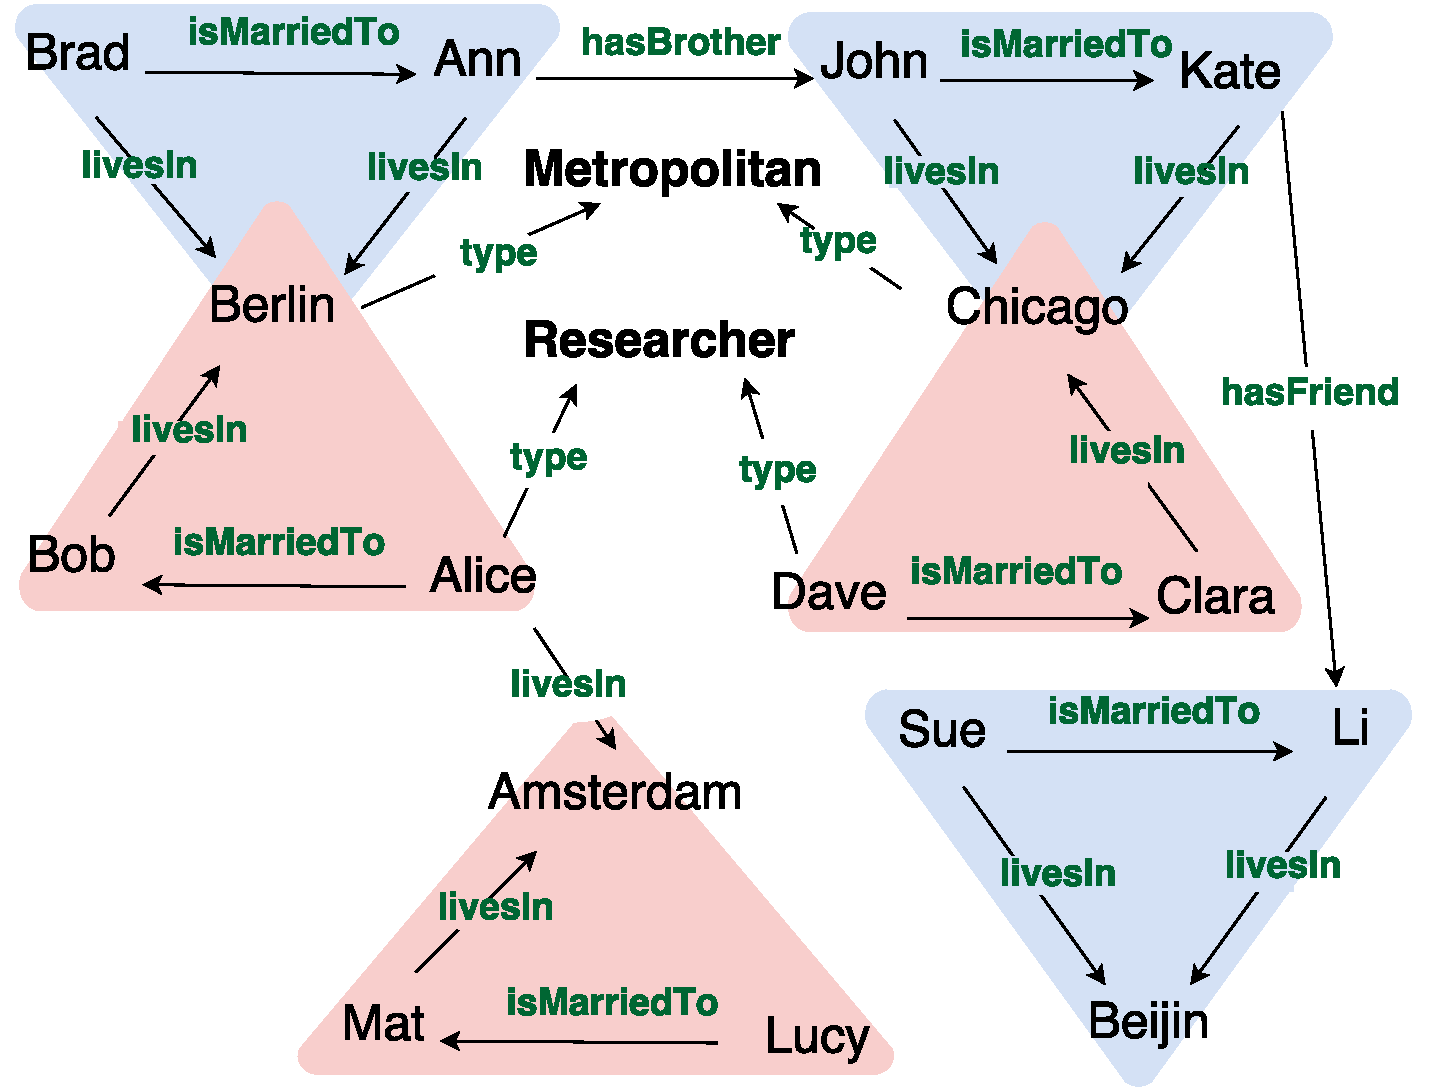
\includegraphics[width=0.75\textwidth]{figures/kg_advanced_col}
\caption{A Visualization of a Knowledge Graph}
\label{fig1.1}
\end{figure}

\section{Challenges}

\textit{Nonmonotonic rule learning}~\cite{ref11, ref40, ref41, ref32, ref42} is to discover a set of rules with exceptions in their bodies (see Chapter \ref{chap:back} for details). Thus, exception mining problem has been addressed in this area. However, the state-of-the-art nonmonotonic ILP algorithms cannot be directly applied to our problem due to the following reasons:
\begin{itemize}
\item First, hardly can the \textit{target relations} be defined because we do not know which parts of the graph need to be extended. A naive solution to this issue is to mine all possible rules for the available predicates in the KG. However, this solution is computationally expensive due to the large number of facts in the original KGs.
\item Second, ILP systems usually exploit positive and \textit{negative examples}. While positive examples are available in our work, negative ones are not given. Besides, the latter are difficult to collect because we sometimes cannot differentiate between wrong and unseen triples and there are a lot of facts in KGs. Thus, a simple approach to overcome this is to discover rules from solely positive facts.
\item Finally, the \textit{language bias} is not easy to define since the schema of the original data is not given. To tackle this, we assume the specific form of the positive rules in Chapter~\ref{chap:system}.
\end{itemize}

To overcome the above obstacles, exploratory data mining solution is a suitable choice. The authors in~\cite{ref12} propose association rule mining methods to explore Horn positive rules, and then revise them by inserting exceptions or negated atoms in their bodies to improve the predictive quality of the rules. However, this approach only works on flattened presentation of a KG, that is, a collection of unary facts.

\section{Goals}

We conduct a research in this thesis with the aim to:

\begin{itemize}
\item Propose a theory to explore interesting and informative nonmonotonic rules.
\item Build an efficient system in terms of run time to generate exceptions from a large collections of facts.
\item Use this tool to verify experimental results and support the theory.
\end{itemize}

\section{Contributions}

This thesis is an extension of the work where KGs are in their natural form~\cite{ref12}. More specifically, we want to mine rules with exceptions from a set of relational facts in KGs treated under OWA. The knowledge completion problem is transformed to \textit{theory revision} one, in which \textit{nonmonotonic rules} are explored given an original KG and Horn rules. The positive rules can be found by using off-the-shell tools for association rule learning. Besides, we expect that the quality of revised rules is better than that of original positive ones with respect to conviction measure[cite???]. There are four steps in our system as follows:

\begin{itemize}
\item First, for each positive rule, we try to find normal and abnormal sets, that is, set of instances that follow and do not follow a given rule, respectively.
\item Second, we mine exception witness sets, that is, set of unary or binary relations that can eliminate abnormal instances. For example, \textit{Researcher} is an exception example for the rule $r1$ based on the KG in Figure~\ref{fig1.1}.
\item Third, we add exceptions to the Horn rules in the form of a single negated atom and define a measure to assess the quality of the obtained revisions. The interaction between revised rules is taken into consideration in our approach by an importantly novel concept of \textit{partial materialization}.
\item Finally, exceptions are ranked based on the proposed measures and the best revision of a particular rule is expected to have both descriptive and predictive qualities.
\end{itemize}

The contributions of this thesis are four-fold:

\begin{itemize}
\item We introduce a framework to revise and improve quality of positive rules.
\item We propose a method for finding exception candidates, assessing their quality and ranking them based on the conviction measure. With the novel concept of \textit{partial materialization}, the cross-talk between the revised rules is taken into account.
\item We implement a system that mines exceptions from a KG and a set of Horn rules. Also, a dataset is built for testing.
\item We conduct experiments with YAGO3 and IMDB datasets to test the above-mentioned methodology and the partial materialization concept.
\end{itemize}

\section{Structure}

The outline of this thesis is as follows. Chapter~\ref{chap:relwork} describes related work and presents the literature review. Chapter~\ref{chap:back} provides background and preliminaries for nonmonotonic logic programs and relational association rule learning. Chapter~\ref{chap:frame} presents the rule learning problem that we are trying to tackle and describes our methodology. Chapter~\ref{chap:system} contains the system overview, implementation details and optimization. Chapter~\ref{chap:eval} indicates dataset construction, experimental results, their analysis and interpretation. Finally, Chapter~\ref{chap:conclusion} is a conclusion for the thesis.